\documentclass[tikz,border=3pt]{standalone}
\usetikzlibrary{arrows.meta}
\usepackage{amsmath,bm}
\let\boldsymbol\bm
\begin{document}
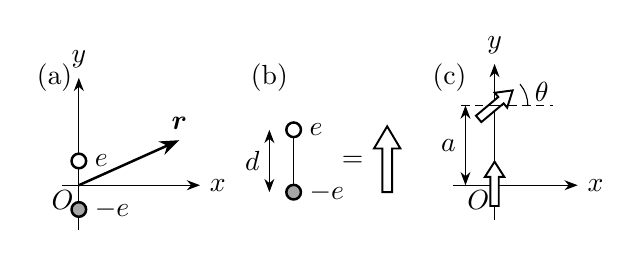
\begin{tikzpicture}[scale=0.88,>=Stealth,line width=0.9pt]
  % (a)
  \begin{scope}[xshift=0cm]
    \node at (-0.35,1.55) {(a)};
    \draw[line width=0.4pt,->] (-0.25,0) -- (1.75,0) node[right] {$x$};
    \draw[line width=0.4pt,->] (0,-0.65) -- (0,1.55) node[above] {$y$};
    \node[below left,inner sep=1.5pt] at (0,0) {$O$};
    \draw[fill=white] (0,0.35) circle (3.0pt);
    \node[right,xshift=2pt] at (0,0.35) {$e$};
    \draw[fill=black!35] (0,-0.35) circle (3.0pt);
    \node[right,xshift=2pt] at (0,-0.35) {$-e$};
    \draw[->] (0,0) -- (1.45,0.65) node[above] {$\boldsymbol{r}$};
  \end{scope}

  % (b)
  \begin{scope}[xshift=3.1cm,yshift=0.35cm]
    \node at (-0.35,1.20) {(b)};
    \draw[line width=0.6pt] (0,-0.45) -- (0,0.45);
    \draw[fill=white] (0,0.45) circle (3.0pt);
    \node[right,xshift=2pt] at (0,0.45) {$e$};
    \draw[fill=black!35] (0,-0.45) circle (3.0pt);
    \node[right,xshift=2pt] at (0,-0.45) {$-e$};
    \draw[line width=0.4pt,<->] (-0.35,-0.45) -- (-0.35,0.45) node[midway,left] {$d$};
    \node at (0.85,0) {$=$};
    % 白抜き矢印
    \draw[line width=0.7pt,fill=white] (1.28,-0.45) -- (1.42,-0.45) -- (1.42,0.18) -- (1.54,0.18) -- (1.35,0.50) -- (1.16,0.18) -- (1.28,0.18) -- cycle;
  \end{scope}

  % (c)
  \begin{scope}[xshift=6.0cm]
    \node at (-0.65,1.55) {(c)};
    \draw[line width=0.4pt,->] (-0.6,0) -- (1.2,0) node[right] {$x$};
    \draw[line width=0.4pt,->] (0,-0.5) -- (0,1.75) node[above] {$y$};
    \node[below left,inner sep=1.5pt] at (0,0) {$O$};
    % 原点の双極子（+y向き）
    \draw[line width=0.7pt,fill=white] (-0.06,-0.30) -- (0.06,-0.30) -- (0.06,0.12) -- (0.14,0.12) -- (0,0.34) -- (-0.14,0.12) -- (-0.06,0.12) -- cycle;
    % (0, a) の双極子（x軸から角度 theta = 40度）
    \begin{scope}[shift={(0,1.15)},rotate=-50]
      \draw[line width=0.7pt,fill=white] (-0.06,-0.30) -- (0.06,-0.30) -- (0.06,0.12) -- (0.14,0.12) -- (0,0.34) -- (-0.14,0.12) -- (-0.06,0.12) -- cycle;
    \end{scope}
    % 水平補助線と角度 theta
    \draw[line width=0.4pt,densely dashed] (0,1.15) -- (0.85,1.15);
    \draw[line width=0.4pt] (0.48,1.15) arc[start angle=0,end angle=40,radius=0.48];
    \node at (0.68,1.35) {$\theta$};
    % 距離 a
    \draw[line width=0.4pt,<->] (-0.42,0) -- (-0.42,1.15) node[midway,left] {$a$};
    \draw[line width=0.4pt,densely dashed] (-0.48,1.15) -- (0,1.15);
  \end{scope}
\end{tikzpicture}
\end{document}
